\documentclass{article}
\usepackage{hyperref}
\usepackage{pgfgantt}
\usepackage{graphicx}
\usepackage{caption}
\usepackage{microtype}

\graphicspath{ {./Images/} }

\begin{document}

\title{Advanced Computer Graphics}
\author{Oliver Eisenberg}
\maketitle
\tableofcontents
\twocolumn

\section{Introduction}
Raytracing is rendering technique that determines visibly and colour objects in a scene. The technique revolves around tracing rays, from the eye or camera, through each pixel and calculating colour upon intersection with the closest object. The principles of raytracing an be extended to visualise shadows, reflection and transmission. 

\subsection{Visibility}
\subsubsection{Rays}
Rays are defined parametrically to take advantage of the \textit{t} parameter, this makes determining the object behind and closest to the camera straight forward - as a negative \textit{t} value means that the intersection occurred behind the camera.

\subsubsection{Ray Intersections}
To be able to add an object to a scene, it must support intersection tests with an arbitrary ray. As more complex objects, like a polymesh, use a series of smaller objects covering basic shapes is enough to cover a majority of the cases. The initial coursework code had sphere intersection support and was later expanded to include triangles and planes.
\subsubsection{The Camera}
The camera model allows the scene to rendered around the viewer. It is used to orientate the scene and emit photons, to be able to do this the camera requires knowledge of its position, where the camera is pointing, the up direction and distance to the image plane is.
\subsection{Colour and Shading}
To determine the colour of the pixel that the ray was traced through the closest object has to be identified, therefore all objects in the scene have to be checked before selecting the object. Furthermore the object has to be checked to see if is in shadow, this is done by emitting a shadow ray towards each light in the scene. Intersections found here, mean that the object is in shadow and, for that light source, the colour doesn't have to be calculated. 

\subsubsection{Local lighting}
Local lighting is the illumination of objects direct from the light source(s) in the scene. Objects can reflect lights either diffuse, which gives a matt effect, or specular which acts like a mirror. 

\begin{equation}
I = I_lk_d(N.L)
\captionsetup{justification=centering,margin=0.5cm}
\label{equ:diffuse}
\end{equation}
\begin{equation}
R = I –2.0 \times (I.N) \times N
\captionsetup{justification=centering,margin=0.5cm}
\label{equ:specular}
\end{equation}

As surfaces are not perfectly smooth the Phong approximation was used, this gives an appropriate shine to an object.

\begin{equation}
I = I_lk_S(R.V)^n
\captionsetup{justification=centering,margin=0.5cm}
\label{equ:phong}
\end{equation}

Therefore the total colour calculation, per colour channel, for an ray to object intersection is.

\begin{equation}
I = I_ak_a+ \sum I_{ln}(k_d(N.L) + k_s(R.V)^n)
\captionsetup{justification=centering,margin=0.5cm}
\label{equ:totalColour}
\end{equation}

\subsubsection{Self Shadows}
When computing shadows self-shadowing can occur. This is caused by rounding errors, where, the shadow ray is generated at a starting point from within the original intersecting object. This causes the shadow ray to hit the inner object and declare that pixel as in shadow - even if it may not be. To resolve this issue the new shadow ray is shifted along the direction of the ray by a small amount. 

Testing all objects for shadows can be optimised as, for a single light source, once you found a shadow identifying another doesn't further shadow the pixel. Therefore the loop that checks for shadow can stop at the first occurrence. Further optimisations can be done through the use of a shadow cache. Shadow caching works due to ray coherence where if a ray is being emitted close by to a previously true shadow ray you can assume that ray also in shadow, preventing checking for an intersection.

\subsubsection{Global lighting}
Global lighting is the addition of secondary rays to compute mirror and transmissive surfaces. 

Reflection works by assuming a specular surface is a perfect mirror. Performing the equation \ref{equ:specular} and raytracing the result calculates the reflected colour, this is then added to the original colour calculated prior to reflecting. The cycle of ray generation for secondary rays leads itself to recursion. 

Similarly to reflection, transparency lends to recursion. This is because secondary rays are produced to simulate the movement of flight through a transparent object. To calculate refraction the index of refraction needs to be set on objection initialisation, this constant is used to determine how much the light is slowed when entering the object. Depending on the incident angle and medium the refracting ray will either slow down and bend towards the normal, speed up and bend away from the normal or undergo total internal reflection. This, however, isn't realistic transparency. This is because, for real materials the angle of incidence changes the amount of reflection and refraction that will occur. To account for this a Fresnel Equation is applied.
\begin{equation}
EQn
\captionsetup{justification=centering,margin=0.5cm}
\label{equ:fresnel}
\end{equation}

\section{Labs}
The completion of lab sheets allowed to get familiar with C++ and to start building practical knowledge on raytracing.
\subsection{Lab 1 - Rasterising Lines}
The line drawing function was updated to use an integer based approach using the Bresenhams Line Algorithm. The algorithm is used to draw a straight line, between two points, in a grid.
\subsection{Lab 2 - Reading Models}
The given code in polymesh.cpp was updated to be able to read 3D objects and generate wireframes from \textit{.ply} files of a certain format. There are several different methods to store polymesh objects, these methods have their own advantages and disadvantages. Only the standard method, in which the teapot uses is supported. The teapot dataset is comprised of three header lines, these identify the number of vertices and faces that are contained and are iterated through to populate their respective vectors.

\subsection{Lab 3 - Simple Raytracing}
\subsubsection{Triangle intersection}
To compute triangle intersections the Möller–Trumbore algorithm was used. This was used instead of the method on the \textit{slides} anticipating the requirements for the barycentric coordinates to complete Gouraud shading further in the coursework.

\subsection{Lab 4 - Basic Lighting and Shadows}
Starting to work on lighting prompted further refactoring. In doing so, a scene class was created to create and store all the objects and lighting for the render. All lights belong to the base light class, this allows to predetermine shared variables and functions a light should have and for lights to be stored in a vector using vector<Light>.
\subsubsection{Types of light}
\subsubsection{Spot Lights - Directional lights}
Spotlights were first implemented due to their simplicity. Spotlights are considered to infinitely far from the scene and therefore have no position and all light rays are parallel.

\subsubsection{Point Lights}
The slides refer to two methods to create point lights, with and without an associated direction. As spot lights are directional, point Lights with a constant intensity were implemented. Allows a point light to be placed between objects to cast shadow outwards. This is demonstrated in \ref{fig:pointlight_white}. 
\begin{figure}[h]
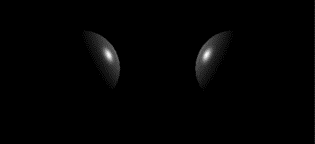
\includegraphics[width=0.5\textwidth]{pointlight}
\captionsetup{justification=centering,margin=0.5cm}
\caption{Simple render to illistrate pointlights}
\label{fig:pointlight_white}
\end{figure}

\subsubsection{Shadows}
Shadows are checked by sending a ray from the hit position to each light in the scene. If an intersection occurs the intensity from that light is removed. This allows for shadows of different intensity depending on the source.

To be able to visualise shadows properly planes were added an 

\section{Optimisations}
Coloured Diffuse
Originally objects had three intensity values representing the three primary colours in addition to the diffuse and specular coefficients. This was later updated to use a material and colour class.

By splitting intensity into colours it allows the addition of coloured lights and control over what coloured objects can reflect this could also benefit possible diffraction and iridescence rendering.
\begin{figure}[h]
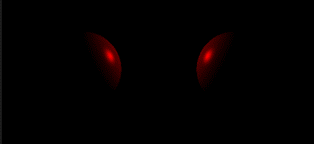
\includegraphics[width=0.5\textwidth]{pointlight_redlight}
\captionsetup{justification=centering,margin=0.5cm}
\caption{Simple render like figure \ref{fig:pointlight_white} but with a red lgiht}
\label{fig:pointlight_red}
\end{figure}

\section{Photon Mapping}
Photon mapping allows to compute global illumination, caustics and precipitation media. 

Some difficulty was encountered when choosing static libraries, this heavily influenced the chosen library to handle KD Trees. The library chosen is \textit{Alglib} was it was written to be added like normal classes where you include the relevant headers and compile the \textit{cpp} files. 
\subsubsection{Random emmition - Lighting}
Lights had to updated with relevant random emisision direction and position functions. Depending on the light 

\subsubsection{Direct lighting}
\begin{figure}[h]
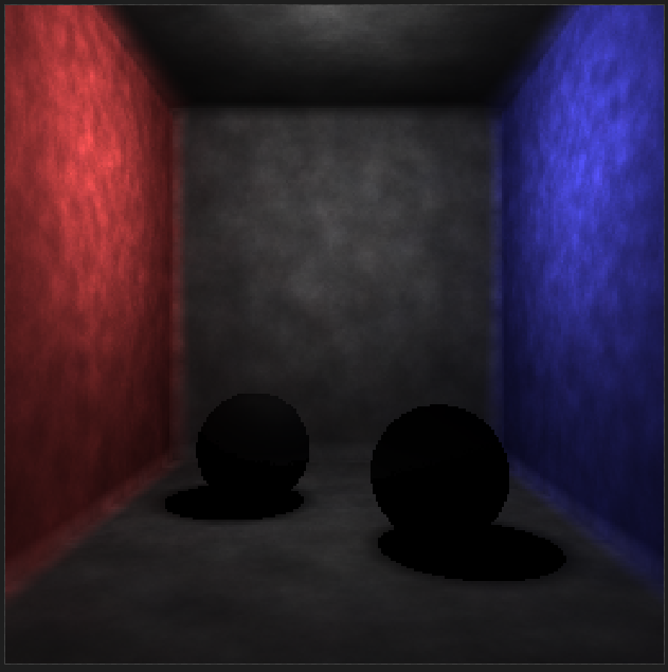
\includegraphics[width=0.5\textwidth]{direct_diffuse}
\captionsetup{justification=centering,margin=0.5cm}
\caption{Render with direct diffuse lighting only}
\label{fig:direct_diffuse}
\end{figure}
\subsubsection{Global illumination}
Takes the initial lighting model and adapts it 

\subsubsection{Specular \& Gloss}
This was straight forward to implement as it is rendered using standard raytracing techniques that were developed during the lab handins. It was slightly updated so that the specular is only displayed when rendering indirectly. 

\subsubsection{Caustics}
Caustics are computationally intensive to calculate using standard raytracing methods but was straight forward to implement using a separate caustic photon map. In a caustic map photons are emitted from the light source to reflective and transmissive objects, later when rendering the caustic map is calculated using a radiance estimate. A caustic map can be filtered prior to rendering to smooth out hard edges - this hasn't been done in my implementation due to time constraints.
\begin{figure}[h]
\centering
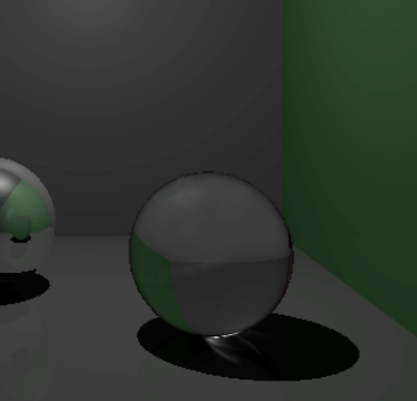
\includegraphics[width=0.5\textwidth]{caustics}
\captionsetup{justification=centering,margin=0.5cm}
\caption{Render with caustics}
\label{fig:caustics}
\end{figure}

\newpage
\begin{appendix}
\listoffigures
\end{appendix}

\bibliographystyle{ieeetr}
\bibliography{./Bibliography}

\end{document}

